\section{Introduction}

    The Higgs Boson sits as the crown jewel of a grand overarching theory of the behaviour of the universe,
        known as the Standard Model of Particle Physics.
    While its recent discovery has shed light on many of its key properties,
        there are still many details of its nature that are as yet uncomfirmed.
    In this chapter, I want to explain what these properties are and how they can be further studied.
    Moreover, I want to justify why the Higgs is so important as to be worth studying in the first place.
    And to understand the importance of the Higgs Boson, one must understand the structure of the Standard Model itself.

    The structure of the following sections will begin with a discussion of the purpose and fundamental structure of the Standard Model.
    I will follow this with an introduction to the mathematical formalism the Standard Model is based around,
        involving Group Theory, the calculus of variations, and symmetry.
    Here I will introduce the reason for the original postulation of the Higgs, what it is, how it works, and how it fits into the Standard Model.
    Finally, I will motivate further study into the Higgs and provide a technique to perform this study.


%Matter and Forces
%I need to discuss the elementary particles and their organization before I can really discuss the gauge fields.
%Might as well do it here first and foremost
\section{The Standard Model of Particle Physics}
    
    At its core, the Standard Model of Particle Physics is a description of the behaviour and interaction of matter.
    First and foremost then, I want to discuss what this matter actually is.
    All matter can be described as a specific type of elementary particle called a fermion,
        defined by the fact that it contains no discernable substructure and possesses an intrinsic spin of 1/2.
    These particles all have different masses, and are able to interact with each other through three ``fundamental interactions''.
    The three fundamental interactions (more commonly called ``Fundamental Forces'') are known as
        the Electromagnetic, Weak, and Strong interactions (gravity is entirely absent in the Standard Model).
    All the interactions have an associated ``charge'' which can be ascribed to different particles,
        and which govern how strongly that particle can interact with similarly charged particles.
    The various fermions are distinct largely because of the charges they carry.

    \begin{figure}[h!]
        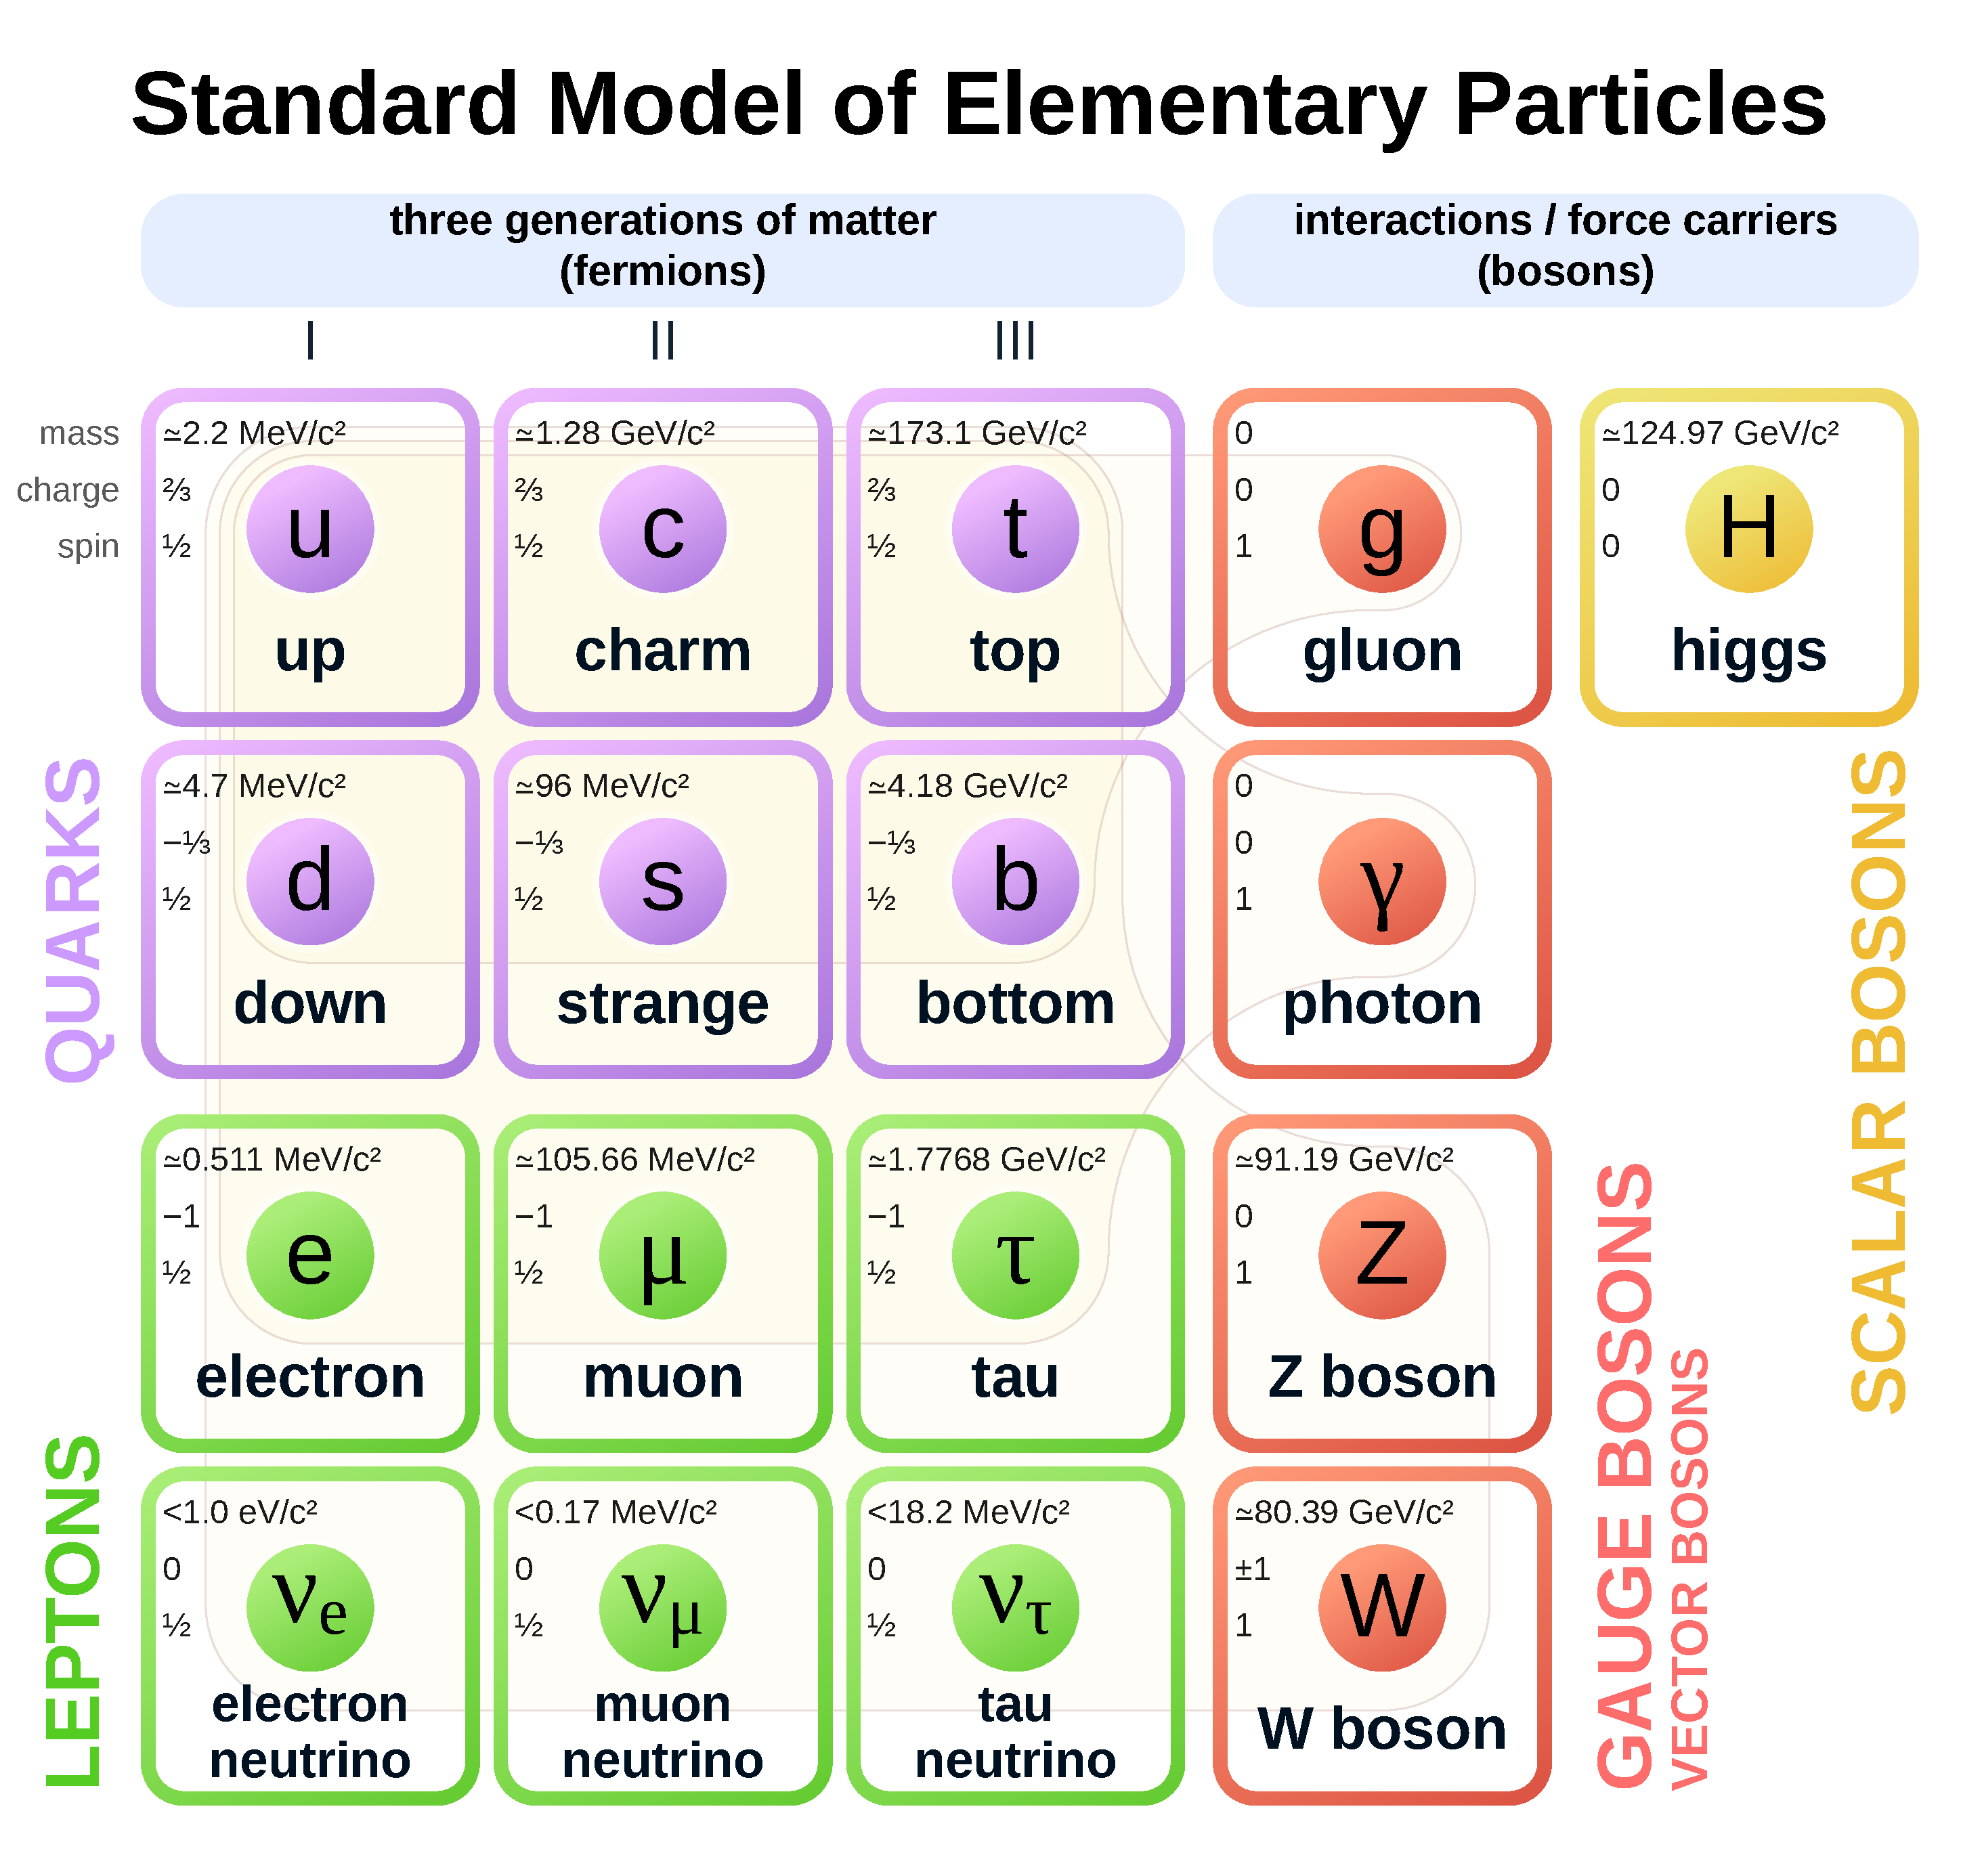
\includegraphics[width=\linewidth,height=\textheight,keepaspectratio]{theory/Standard_Model_of_Elementary_Particles}
        \caption{I'm probably going to need to find something else since this came from wikipedia. I just wanted a placeholder}
        \label{fig:sm_particles}
    \end{figure}
        

    There are twelve distinct elementary fermions (see Figure \ref{fig:sm_particles}),
        which are split evenly into two subgroups, called quarks and leptons.
    Quarks have a charge of 1 with the Strong interaction,
        while leptons have a charge of 0 (and thus cannot interact via the Strong Interaction at all).
    Both classes of particles, quarks and leptons, are divided into three ``generations'' of progressively heavier particles.
    Each generation thus consists of two quarks and two leptons.
    These pairs, called ``doublets'', behave the same across all generations.
    Among the quarks, every generation contains a doublet of an up-type quark (Up, Charm, Top) with electromagnetic charge of 2/3,
        and a down-type quark (Down, Strange, Bottom) with EM charge of -1/3.
    For leptons, each doublet consists of a particle with EM charge of -1, and a neutrino with EM charge of 0.

    In addition to the fermions, there is also an entirely seperate class of particles, called gauge bosons,
        which play a fundamental role in the aforementioned interactions.
    However, the nature of these particles will be discussed later.
    Now, with the enumeration of the various particles complete, it is time to begin the discussion of the Standard Model itself,
        which will serve to explain how these fermions interact with each other.



\section{Composition of Matter: Fields and Dirac Spinors}
    I'm actually starting to wonder if I should scrap this entire section and just merge the basic description of fields,
        as well as a brief mention of the Dirac equation, into the prior section.
    I don't think I'm going to go into detail about the weak-fermion coupling,
        so I don't really need to describe left/right fields, so I don't really need to break down the structure of
        the dirac and klein gordon equations.
    I might even just move the klein gordon equation introduction over to the Higgs section.

    %Fields are a thing.
    The description of matter is governed by the formalism of Quantum Field Theory, which describes particles as pertubations of an overall particle \textit{field}.
    %They're kinda like quantum waves, but not.
    A particle field $\varphi$, describes every particle of the same type at once,
        and particle states $\ket{\varphi}$ correspond to the number of that kind of particle that exists at a given moment.
    The equation of motion used to describe a field varies depending on the properties of the field.
    For a scalar (spinless) field, \phi, the equation of motion just comes from the relativistic mass-four-momentum relation $p^2=m^2$,
        but repurposed for a quantum field.
    This is the Klein-Gordon Equation
    \begin{equation} \begin{split}
        p^2 \phi = m^2 \phi
        \\(p^2 - m^2) \phi = 0
    \end{split} \end{equation}
    Recalling the covariant, natural units, quantum mechanical definition of momentum as $p^u = i\partial^u$,
        this can also be written as
    \begin{equation} \begin{split}
        (p^2 - m^2) \phi = 0 \rightarrow (\partial^\mu \partial_\mu + m^2) \phi = 0
    \end{split} \end{equation}

    The Klein-Gordan Equation will be used later when describing the Higgs Field,
        but first I will use it here as the foundation for the equation of motion required for a spinor field.
    For spinor fields, the equation of motion is the Dirac Equation,
        formulated to be a first-order equation (i.e.\ linear in $p$).
    \begin{equation}
        (\gamma^\mu p_\mu - m I) \psi = 0
        (i\gamma^\mu \partial_\mu  - m I) \psi = 0
    \end{equation}

    The issue with creating a first-order equation in $p$ is that $p_\mu$ is a vector, which means it cannot be merely added to the scalar $m$.
    The key feature of the Dirac Equation which addresses this is the inclusion of the \textit{gamma matrices}, $\gamma^\mu$.
    $\gamma^\mu$, is a vector of four matrices, each of size 4x4 (note that $m$ is in turn multiplied by a 4x4 identity matrix $I$).
    There are many different conventions for the exact structure of the matrices,
        but the main requirement is that they all multiply together with very specific commutation rules.
    The technical description of this property is that the gamma matrices must
        anti-commute as $\{\gamma^u, \gamma^\nu\} = 2g^{\mu \nu}\times I$,
        where $g^{\mu\nu}$ is the minkowski metric.
    In practical terms, the goal is just to ensure that when the Dirac Equation is multiplied by its conjugate,
        the product returns back to the Klein-Gordan Equation.
    \begin{equation} \begin{split}
        (\gamma^\nu p_\nu + m I) (\gamma^\mu p_\mu - m I) \psi = 0
        \\ (\gamma^\nu \gamma^\mu p_\nu p_\mu - m \gamma^\nu p_\nu + m \gamma^\mu p_\mu - m^2 I) \psi = 0
        \\ (\gamma^\nu \gamma^\mu p_\nu p_\mu - m^2 I) \psi = 0
        \\ (g^{\mu \nu} I p_\nu p_\mu - m^2 I) \psi = 0
        \\ (p^\mu p_\mu - m^2 ) \psi = 0
        \\ (p^2 - m^2) \psi = 0
    \end{split} \end{equation}
    Where the anticommutation relation has been used in the fourth line to eliminate all the momentum cross terms.




    %Fields don't describe a single particle, but all particles of the same type at once.
    %Field states are just a count of how many of that particles exist at a given time.
    %Scalar particles are described by Klein Gordon Equation.
    %Spin 1/2 particles are described by dirac equation.
    %It's first order in p, but this requires the gamma matrices.
    %Matrices take many forms, but one of the most revealing is the Weyl, or Chiral, form.
    %Do some math to show fields in chiral form, to show Chirality.


    %It takes from quantum mechanics the uncertainty principle, and from relativity the mass/energy equivalence 
    %It takes from quantum mechanics the wave-like description of position and momentum, along with the uncertainty principle.
    %From special relativity it incorporates the equivalence of space and time, the constance of the speed of light,
    %    and the exchange between mass and energy.
    %Combining the energy/time uncertainty principle with mass/energy equivalence in particular
    %    has the outcome that the number of particles for a given system need not remain constant.
    %To account for this, particles are not described as waves as with the Schrodinger Equation, but rather as ``fields''.
    %A fermion field, $\psi$, does not describe a single particle, but rather all possible fermion for the same kind of particle.
    %For instance, there is a seperate fermion field to describe electrons, up-quarks, and so forth.

    
    describe gamma matrices

    describe anti particle psi bar

    describe chiral representation
    

    %What is the Universe made of (If you stick to this format at all, keep this section brief):

    %%Position and Momentum: Quantum Mechanics
    %   The position and momentum of that matter:
    %       Described via the Canonical Commutation Relation and the formalism of Quantum Mechanics
    %       (explain 'h' here?)
    %   Describe basic function of schrodinger equation and why it fails

    %%Space and Time: Special Relativity
    %   The space-time in which that matter resides: described by the Minkowski Metric Tensor.
    %    Explain what the metric tensor means and maybe covariant notation,
    %    as well as mass-energy-momentum equivalence,
    %    and also the speed of light
    %    Reformat schrodinger equation as klein gordon and show how this also fails


    %%Particles and Fields: Quantum Field Theory
    %   A description of how the position of matter can change: Described by the Dirac Equation.
    %    A unification of Quantum Mechanics and Special Relativity
    %    (maybe go through the derivation, starting from schrodinger -> klein-gordon -> dirac and why each fails)
    %    Describe Weyl Spinors and Chiral representation (peskin pg 64)



\section{Generating Motion: Group Theory and Transformations}

    The Dirac Equation provides a description of matter.
    The next key piece of the Standard Model is a description of motion itself.
    For this, I will need to introduce Group Theory.

    A function can be altered using a \textit{transformation operator}.
    A simple example of this would be a function $x(t)$, 
        which (assuming constant velocity) can be transformed into a time $\Delta t$ in the future as
    \begin{equation}
    x(t) \rightarrow x'(t) = x(t) + v \Delta t
    \end{equation}
    Noting that $v$ is just $\frac{d}{dt} x(t)$, this can be rewritten as
    \begin{equation}
    x(t) \rightarrow x'(t) = x(t) + \Delta t \frac{d}{dt} x(t) = \left(1+\Delta t \frac{d}{dt}\right) x(t)
    \end{equation}

    This term $\left(1+\Delta t \frac{d}{dt}\right)$ is the classical time-translation operator.
    Notice the assumption of \textit{constant velocity} though.
    If velocity were not constant, this operator would be invalid, except for in the specific case in which $\Delta t$ is infinitesimal.
    \begin{equation}
    x(t) \rightarrow x'(t) = \lim_{\delta t \to 0} \left(1+\delta t \frac{d}{dt}\right) x(t)
    \end{equation}

    To produce a more general finite operator I can apply the infinitesimal operator an infinite number of times
    \begin{equation} \begin{split}
    x(t) \rightarrow x'(t) &= \lim_{\delta t \to 0} \left(1+\delta t \frac{d}{dt}\right)\left(1+\delta t \frac{d}{dt}\right)\left(1+\delta t \frac{d}{dt}\right)...\ x(t)
    \\x(t) \rightarrow x'(t) &= \lim_{N \to \infty} \lim_{\delta t \to 0} \left(1+\delta t \frac{d}{dt}\right)^N x(t)
    \\x(t) \rightarrow x'(t) &= e^{\Delta t \frac{d}{dt}} x(t)
    \end{split} \end{equation}

    Where $\Delta t$ is again a finite time transformation,
        and I have compressed the infinite product of terms using the power series expansion of the exponential function.
    In order to use this classical operator in quantum field theory, it must have a complex factor `$i$' associated with it,
    \begin{equation} \begin{split}
    x(t) \rightarrow x'(t) = e^{i\Delta t \frac{d}{dt}} x(t)
    \end{split} \end{equation}

    Returning to Dirac Fields, which are functions of four-position $x_\mu$, this same transformation can be used
         with the minor adjustment of changing the total derivative to a partial derivative in time, $\frac{partial}{\partial t} = \partial_0$
    \begin{equation} \begin{split}
    \psi(x) \rightarrow \psi'(x) = e^{i\Delta x^0 \partial_0} \psi(x)
    \end{split} \end{equation}

    Meanwhile, the Dirac anti-particle field transforms with a negative sign as
    \begin{equation} \begin{split}
        \psibar(x) \rightarrow \psibar'(x) = e^{-i\Delta x^0 \partial_0} \psibar(x)
    \end{split} \end{equation}
    
    The time translation operator is but one of a myriad of different tranformation operators.
    However, all of the transformation operators that will be used here will all take a form very similar to this one,
        appearing something like

    \begin{equation} \begin{split}
        \psi(x) \rightarrow \psi'(x) = e^{ q \cdot \mathcal{F}_q } \psi(x)
    \end{split} \end{equation}

    where $\mathcal{F}_q$ is the transformation \textit{generator} (e.g.\ $i\partial_0$),
        and $q$ the amount to transform by (e.g.\ $\Delta t$).

    These transforms all fall under a larger realm of mathematics known as Group Theory,
        and are in turn called ``group transformation''.
    The basic definition of a ``group'' is a set of elements which can be ``multiplied'' according to some rule,
        and which satisfies the four conditions of\cite{Cheng_book}:
    \begin{itemize}
        \item Closure - the product of any two elements of the group are still in that group;
        \item Associativity - $(a \times b)\times c = a\times(b \times c)$;
        \item Identity - there is some element in the group $I$ for which $I \times a=a$;
        \item and Inversion - every element $a$ has an inverse $a^{-1}$ such that if $b \times a = c$ then $c \times a^{-1} = b$.
    \end{itemize}

    It should be relatively simple to see that time translation operations satisfy each of these.
    Additional classifications for groups are whether a group is discrete or continuous,
        and whether a group is ``Abelian'' (commutative) or ``non-Abelian'' (non-commutatitve).
    Time translations are continuous (one can tranlate by an infinitesimally small amount of time),
        and are Abelian (the order that the translation are applied does not matter).
    An example of a non-Abelian group would be that of three-dimensional rotations (formally called the $SO(3)$ group),
        as applying rotations in a different order can lead to a different final product.

    As a final point regarding Group Theory, is the absolutely crucial idea of \textit{symmetry}.
    If a system can be transformed under a group transformation and remain overall unchanged,
        then that system is said to be invariant, or symmetric, under that group.
    In a very deep sense, Group Theory and group symmetry are the driving forces behind the entire Standard Model,
    As will be seen in the coming sections,
        the motion of the Standard Model is ultimately described by Group Theory,
        its interactions defined by Group Theory,
        and its entire organizational structure ultimately rooted in Group Theory.

\section{Restricting Motion: The Lagrangian and Symmetry}
    
    The Dirac Equation describes the equation of motion of a single field,
        but what is required is a way to describe the interactions of \textit{many} fields.
    For this, the Standard Model makes use of the Principle of Least Action,
        also known as the Lagrangian Formulation\cite{Halzen_book}.
    The idea of the Principle of Least Action is to construct an overall description of all aspects of a system,
        called the Lagrangian, $\Lag$.
    One can then find the ``path'' of this Lagrangian which minimizes the ``Action'', $\mathscr{A}$
    \begin{equation} %TODO: double check this!!
        \mathscr{A} = \int \Lag d^4 x
    \end{equation}

    This minimization is performed using the four-dimension Euler-Lagrange equations
    \begin{equation}
        \partial_\mu \frac{\partial \Lag}{\partial_\mu \varphi } - \frac{\partial \Lag}{\partial \varphi} = 0
    \end{equation}
    which yields the equations of motion of the interacting particles.

    All of the physics of the Standard Model is inscribed within the Standard Model Lagrangian.
    The construction of this Lagrangian will be the focus of most of the rest of the chapter.
    To begin then, what physics \textit{does} the Lagrangian need to encode?
    Paraphrasing Murray Gell-Mann, ``that which is not forbidden, is \textit{mandatory}.''
    That is to say, that any physics which is not expressly prohibited, must automatically be allowed.
    Formulation of the Standard Model Lagrangian must therefore start with an enumeration of restrictions,
        given in the form of a series of groups that the Lagrangian must remain symmetric under.
    Specifically, the Lagrangian must remain symmetric under ten transformations,
        collectively reffered to as the Poincare Group.
    Four of these transformations correspond to the space-time translations,
        three to spatial rotations, and the remaining three to space-\textit{time} rotations,
        also known as Lorentz Transformations (also known as just changing velocity).

    The Lagrangian of a Dirac field satisfying these symmetries takes the form
    \begin{equation}
        \Lag = \psibar (\slashed{p} - m) \psi = i \psibar \slashed{\partial} \psi - m \psibar \psi
    \end{equation}
    Applying the Euler-Lagrange equations to this equation will seperately return the Dirac Equation
        for the fermion and anti-fermion fields, as it should.

    As there are many different kinds of fermions, the Lagrangian can be expanded to include all of them
    \begin{equation}
        \Lag = \bar{e} (\slashed{p} - m) e
        + \bar{\mu} (\slashed{p} - m) \mu
        + \bar{\tau} (\slashed{p} - m) \tau
        + \bar{u} (\slashed{p} - m) u
        + ...
    \end{equation}

    Although this equation qualifies as a valid description of the behaviour of fermions,
        there is a glaring flaw with it: the fields it describes are all completely independent of one another.
    None of the fields are able to interact with each other.
    In its current form, the Lagrangian proposes that particles, given some initial momentum,
        will persist along the same trajectory forever, unable to affect or be affected by any other particle.
    The Lagrangian has succesfully constrained the range of allowed physics,
        but it has done so to such a degree that the described physics are now practically static.
    Clearly this is not a satisfactory description of the universe, full of dynamic interactions as it is.
    The resolution to this issue is, counter-intuitively, to enforce yet \textit{more} symmetry requirements.



    %Should I also discuss renormalizability? (Peskin pg 80/101djvu)
    %Basically, all lagrangians must be renormalizable.
    %Renormalizability just means that the lagrangian doesn't explode from the unconstrained nature of virtual particles.
    %So infinite-mass virtual particles should not break a renormalizeable lagrangian.


\section{Transferring Motion: Gauge Symmetry}
    Gauge Transformations are ones where the transformation is imposed differently at each point in spacetime.
    Trying to impose a constraint on the Lagrangian that it be symmetric under gauge transformations would surely cause all manner of complications.
    Obviously, this is exactly what nature seems to have chosen to do.

    Gauge symmetries; U1, SU(N).
    The effects of imposing gauge symmetries on the Lagrangian, and the advent of the gauge bosons and their forces.
    how do gauge bosons come out from symmetries.

    U(1) is phase transforms

    SU(2) is based on 2x2 pauli matrices and thus requires pairing generations of particles together;
        so up and down-type quarks are paired together and charged leptons with neutrinos.
    It treats left handed fields as these doublet pairs,
        but works in "singlet representation" (which means it basically is just gone) for right-handed fields

    SU(3) is based on a 3x3 structure constant, and thus acts on all three "generations" of quarks as one 3x1 vector.
    It is a singlet (read, it literally doesn't matter) for leptons.
    
    \cite{Osborn_notes}
    \cite{Peskin_book}
    \cite{Halzen_book}

